\documentclass[./main.tex]{subfiles}
\begin{document}
\chapter{三维空间的向量代数}

\section{向量的引入}

我们生活在三维欧式空间里, 为了解决具体的问题, 我们会人为地建立理想的直角坐标系辅助研究. 而在本章节我们不着急于坐标系的简历, 而是把注意力放在最基本的向量代数上, 以此训练我们的抽象思维. 

\section{向量定义与线性运算}

按照讲义中定义, 我们把三维欧氏空间中既有大小也有方向的量称为向量. 向量的基本性质与运算实际上我们并不陌生, 所以笔者只是将其简单带过. 而在这定义当中, 最值得注意的是\textit{三维欧氏空间}这一限制. 这里原始讲义并未向我们阐明欧式空间到底是什么, 我们似乎可以把欧式空间看做自欧几里得《几何原本》公理所构建的几何化的世界. 实际上, 我们课程的学习以及各类课程目标的设置上并不要求我们学会古典的公理化的几何证明, 更重要的是在欧式空间与其他空间上定义的``向量''又有什么区别. 

一个经典的例子是``电流''既有大小也有方向, 但很明显它并不符合我们对向量的直观认识, 今后我们对向量定义建立的求和, 内积等运算也并不适用, 从这个例子我们尝试一窥``向量''特意强调在欧式空间上定义的原因. 

我们知道向量代数的建立是为了解决实际问题, 欧氏空间是数学家为更好的模拟解析现实空间量身构建的理论. 对数学学习者, 欧氏空间保有从\(V\times V\)到\(\mathbb{R}\)的内积映射, 这使得欧氏空间有别于一般的线性空间. 在1.4章节我们引入内积与外积时我们还会继续讨论这一点. 

向量还具备如下性质: 存在逆向量, 加法满足三角形法则, 随后我们可以推导出在这样的向量空间中加法与数乘都保持交换律与结合律. 结合我们高等代数的知识我们清楚, 倘若我们参考高等代数中线性空间的定义, 我们也完全可以定义明白本自然段向量的若干性质. 事实上笔者认为, 这里如果把向量定义为一个保持1.4中直观想象下内积映射的三维线性空间中的元素, 或许可以避免很多定义的含混. 

\section{向量的位置关系}

我们如上文定义向量, 所求即为借助向量研究物质世界, 借助例子我们发现研究向量之间的位置关系是必要的. 当然我们知道一般线性空间中的元素一般无法考查位置关系这一概念, 在本书三维欧式空间中的向量我们可以讨论位置关系得益于在1.4引入的向量内积这一概念. 

我们可以通过平移后共线/共面来定义向量的共线/共面, 但笔者更愿意从数乘关系等代数化的角度引入这些概念, 即: 
\begin{theorem}[共线定理]
    \(\mathbf{a}, \mathbf{b} \)共线当且仅当存在唯一实数\(\lambda\)满足
\[\mathbf{a} =\lambda \mathbf{b}.\]
\end{theorem}
\begin{theorem}[共面定理]
\(\mathbf{a}\)与\(\mathbf{b}\)为不共线两向量, 则\(\mathbf{c}\)与\(\mathbf{a}, \mathbf{b}\)共面当且仅当存在唯一的实数对\(\lambda ,\mu\)满足
\[\mathbf{c}=\lambda \mathbf{a} +\mu \mathbf{b}.\]
\end{theorem}
至于垂直关系, 笔者认为从下一节才可以严谨引入. 
\section{向量的内积与外积}
前文已经介绍, 如果我们引入代数的想法去观察矢量, 我们可以对矢量的定义与性质有更清晰的看法. 同样的, 对于内积的引入, 我们从分析的角度知道是为了让我们所研究的矢量具有一个从\(V\times V\)到\(\mathbb{R}\)的映射, 使得对矢量的研究可以更好的帮助我们研究物质世界. 

我们定义向量的\textit{内积}为:
\[\mathbf{a}\cdot\mathbf{b}=\left |\mathbf{a} \right | \left | \mathbf{b} \right | \cos  \left \langle \mathbf{a},\mathbf{b} \right \rangle,\]
其中\(\left \langle\mathbf{a},\mathbf{b} \right \rangle\)为向量\(\mathbf{a}\)与\(\mathbf{b}\)的夹角. 这里对夹角与内积的定义依旧依托几何上的角度关系, 当我们学习了第二章之后以坐标运算作为内积的原始定义可能更加自然. 

内积的定义里使得我们直观上夹角为直角的向量内积为零, 换言之, 如果我们先以坐标运算定义内积, 我们便可以通过内积值为零定义垂直关系, 而两向量内积值与模长的比取反三角函数, 也可以为一系列三维数组定义夹角关系. 从这里我们可以看出\textbf{三维欧氏空间中内积的存在是其可以度量角度关系, 从而有别与一般线性空间, 更好拟合物质世界的根本特征}

内积满足乘法交换律, 与数乘的交换律, 结合律, 以及乘法分配律
我们仅对分配律进行证明. 对于向量\(\mathbf{a}, \mathbf{b}\)在平移至下图情形, 其中\(\overrightarrow{OM}\)即为向量\(\mathbf{c}\). \(A_1\)为\(A\)向\(OM\)直线引垂线的垂足, \(\overrightarrow{A_1B_1}\)为\(\overrightarrow{OM}\)平移至始点为\(A_1\)的向量. 我们发现点\(B\)与点\(B_1\)向直线\(OM\)作垂线所得垂足均为点\(N\)故而知道\(\overrightarrow{OA}\), \(\overrightarrow{AB}\)在直线\(OM\)上的投影向量和即为\(\overrightarrow{OB}\)在直线OM上的投影向量, 故而分配律成立. 
\begin{figure}[!ht]
    \centering
    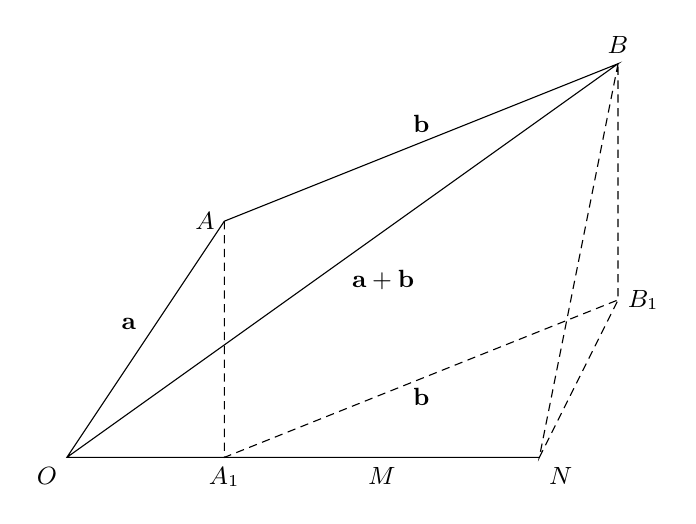
\begin{tikzpicture}
        \node[below] (M) at (4,0){\small\(M\)};
        \draw (6,0)node[below right]{\small \(N\)}--(0,0)node[below left]{\small\(O\)}--node[above left]{\small\(\mathbf{a}\)}(2,3)node[left]{\small \(A\)}--node[above]{\small \(\mathbf{b}\)}(7,5)node[above]{\small \(B\)}--node[below right]{\small\(\mathbf{a}+\mathbf{b}\)}(0,0);
        \draw[densely dashed] (7,5)--(6,0)--(7,2)--(7,5);
        \draw[densely dashed] (2,3)--(2,0)node[below]{\small\(A_1\)}--node[below]{\small\(\mathbf{b}\)}(7,2)node[right]{\small\(B_1\)};
    \end{tikzpicture}
\end{figure}
正如同我们依靠内积更好刻画两个向量的角度, 从而更好研究平面向量问题, 我们对外积的研究也可以帮助我们完成向量维数的扩张. 在有了左手系与右手系的基本知识后, 我们定义两向量的外积 (叉乘) 为一个向量, 向量的模长满足: 
\[\left | \mathbf{a}\times \mathbf{b} \right | =\left | \mathbf{a} \right | \left | \mathbf{b} \right | \sin\langle\mathbf{a},\mathbf{b}\rangle.\]

向量的方向与叉乘两向量垂直, 且依次序\(\mathbf{a}, \mathbf{b}, \mathbf{a}\times \mathbf{b}\)构成右手系. 当然对于\(\mathbf{a}, \mathbf{b}\)平行的特殊情况叉乘为零向量. 

对于叉乘的性质我们也只对分配率简单说明, 即
\[(\mathbf{a}+\mathbf{b})\times\mathbf{c}=\mathbf{a}\times\mathbf{c}+\mathbf{b}\times\mathbf{c}\]

这里我们只需要说明不妨设\(\mathbf{a}\)与\(\mathbf{b}\)在\(\mathbf{c}\)方向上分量大小不影响叉乘结果, 故而可设\(\mathbf{a}\)与\(\mathbf{b}\)垂直于\(\mathbf{c}\), 然后只需证明\(\mathbf{a}\)与\(\mathbf{b}\)也相互垂直时可分配, \(\mathbf{a}\)与\(\mathbf{b}\)不垂直时将\(\mathbf{b}\)分解至\(\mathbf{a}\)与\(\mathbf{c}\times\mathbf{a}\)两方向上即可. 

\section{混合积与双重外积}

我们定义三个向量的混合积为\((\mathbf{a},\mathbf{b},\mathbf{c})\)一个标量, 其中
\[(\mathbf{a},\mathbf{b},\mathbf{c})=\left | \mathbf{a}\times \mathbf{b} \right |\left | \mathbf{c} \right |   \cos\langle\mathbf{a}\times\mathbf{b},\mathbf{c}\rangle\]
 
此时混合积表示三个向量构成的平行六面体的有向面积, 混合积为零也是三向量共面的特征. 

从混合积的几何意义知道混合积具有轮换性, 若是从代数角度构建知识逻辑混合积的轮换性则是由混合积的行列式计算公式得到. 由轮换性又由外积的分配律, 我们知道混合积具有分配律, 此时若向量\(\mathbf{d}, \mathbf{x}, \mathbf{y}, \mathbf{z}\)有\(\mathbf{d}=x\mathbf{a}+y\mathbf{b}+z\mathbf{c}\)
此时由\((\mathbf{d},\mathbf{b},\mathbf{c})=(x\mathbf{a}+y\mathbf{b}+z\mathbf{c},\mathbf{b},\mathbf{c})=(x\mathbf{a},\mathbf{b},\mathbf{c})=x(\mathbf{a},\mathbf{b},\mathbf{c})\)我们便有: 
\[x=\frac{(\mathbf{d},\mathbf{b},\mathbf{c})}{(\mathbf{a},\mathbf{b},\mathbf{c})}.\]

同理, 我们最终得到: \[x=\frac{(\mathbf{d},\mathbf{b},\mathbf{c})}{(\mathbf{a},\mathbf{b},\mathbf{c})}, y=\frac{(\mathbf{a},\mathbf{d},\mathbf{c})}{(\mathbf{a},\mathbf{b},\mathbf{c})}, z=\frac{(\mathbf{a},\mathbf{b},\mathbf{d})}{(\mathbf{a},\mathbf{b},\mathbf{c})}.\]

接下来我们介绍双重外积公式:
\[(\mathbf{a}\times\mathbf{b})\times\mathbf{c}=(\mathbf{a}\cdot\mathbf{c})\mathbf{b}-(\mathbf{b}\cdot\mathbf{c})\mathbf{a}.\]

本公式的证明在书中仍然采取与外积分配律证明完全相同的方法, 从特殊到一般研究该问题. 然而若是我们一开始采取代数的逻辑体系介绍内积与外积, 使用坐标对三维向量进行计算便可以很简便的得出. 这一方面再次证明了代数理论的优越性, 一方面也印证了本章节前言所说的, 本章向量代数的介绍目的是锻炼我们的思维, 达到思维体操的效果. 

我们再取几个例子对混合积与双重外积公式进行实际应用. 

\begin{proposition}
    \[(\mathbf{a}\times \mathbf{b})\times (\mathbf{c}\times \mathbf{d})=(\mathbf{a},\mathbf{b},\mathbf{d})\mathbf{c}-(\mathbf{a},\mathbf{b},\mathbf{c})\mathbf{d}\] 
\end{proposition}
\begin{proof}
    \begin{multline*}
        (\mathbf{a}\times \mathbf{b})\times (\mathbf{c}\times \mathbf{d})=-(\mathbf{c}\times \mathbf{d})\times(\mathbf{a}\times \mathbf{b})\\=-[\mathbf{c}\cdot (\mathbf{a}\times \mathbf{b})]\cdot \mathbf{d}+[\mathbf{d}\cdot (\mathbf{a}\times \mathbf{b})]\cdot \mathbf{c}=(\mathbf{a},\mathbf{b},\mathbf{d})\mathbf{c}-(\mathbf{a},\mathbf{b},\mathbf{c})\mathbf{d}.
    \end{multline*}
\end{proof}
\begin{proposition}
\[(\mathbf{a}\times \mathbf{b})\cdot (\mathbf{c}\times \mathbf{d})=(\mathbf{a}\cdot \mathbf{c})(\mathbf{b}\cdot \mathbf{d})-(\mathbf{a}\cdot \mathbf{d})(\mathbf{b}\cdot \mathbf{c})\]
\end{proposition}
\begin{proof}
    \begin{multline*}
        (\mathbf{a}\times \mathbf{b})\cdot (\mathbf{c}\times \mathbf{d})=(\mathbf{a},\mathbf{b},\mathbf{c}\times \mathbf{d})=(\mathbf{c}\times \mathbf{d},\mathbf{a},\mathbf{b})\\=((\mathbf{c}\times \mathbf{d})\times \mathbf{a})\mathbf{b}=[(\mathbf{c}\cdot \mathbf{a})\mathbf{d}-(\mathbf{d}\cdot \mathbf{a})\mathbf{c}]\cdot \mathbf{b}=(\mathbf{c}\cdot \mathbf{a})(\mathbf{d}\cdot \mathbf{b})-(\mathbf{d}\cdot \mathbf{a})(\mathbf{c}\cdot \mathbf{b})\\=(\mathbf{a}\cdot \mathbf{c})(\mathbf{b}\cdot \mathbf{d})-(\mathbf{a}\cdot \mathbf{d})(\mathbf{b}\cdot \mathbf{c}).
    \end{multline*}
\end{proof}
\end{document}
